%        File: TracerVFlux3rd.tex
%     Created: Fri Feb 03 07:00 AM 2012 M
% Last Change: Fri Feb 03 07:00 AM 2012 M
%
\documentclass[11pt]{report}
\usepackage{amsmath}
\usepackage{amsfonts}
\usepackage{subfigure}
\usepackage{placeins}
\usepackage{graphicx}
\usepackage{listings}
\usepackage{float}
\title{Monotonic Tracer Advection}
\setcounter{secnumdepth}{5}
\setcounter{tocdepth}{5}
\begin{document}
\maketitle

\chapter{Summary}
This document outlines the monotonoic tracer advection implementation within
the MPAS framework. The issues section relates to trying to make this a shared
set of modules that can be used in any core. \\

In the attempt to make the module shared in something like operators, several
issues arose which are also presents along with potential fixes for these
issues.

\chapter{Requirements}

\begin{itemize}
	\item Shared Advection Routines
	\item Horizontal and Vertical Advection of Tracers or Scalars
	\item Monotonic Advection
	\item FCT
\end{itemize}
\chapter{Formulation}

The tracer advection equation can be written as follows:
\begin{equation}
	\frac{\partial Q_i}{\partial t} = - (\nabla \cdot \vec{V} Q_i) + F_{Q_i}
	\label{eq:cont_tracer_adv_full}
\end{equation}

where $Q$ represents a weighted tracer quantity, $\vec{V}$ represents the 3-D velocity
vector, and $F_{Q}$ represents the source and sink terms for this tracer. \\

In the ocean, we use the definition that ${Q} = h q$ where $h$ is the fluid
thickness field, and $q$ is the tracer quantitiy, which can be a vector representing various tracers.

Because this formulation relates to tracer advection in the ocean, we assume $F_{Q} = 0$, and (\ref{eq:cont_tracer_adv_full}) reduces to:
\begin{equation}
	\frac{\partial h q}{\partial t} = - (\nabla \cdot \vec{V} h q)
\end{equation}direction. \\

Following the notation of Dutton (1986) we define
\begin{equation}
	(\nabla \cdot \vec{V} h q) = \nabla \cdot (\vec{V_H} h q) + \frac{\partial (w h q)}{\partial z}
\end{equation}
where $V_H$ is the horizontal component of velocity, and w is the vertical component of velocity..

\section{Horizontal Advection}
This section deals with the horizontal tracer advection, which can be described by the following equation.
\begin{equation}
	\frac{\partial h q}{\partial t} = - \nabla \cdot (V_H h q)
	\label{eg:horiz_adv_cont}
\end{equation}

The figure below is used to help visualize the layout of data within an MPAS grid.
\begin{figure}[H]
	\centering
	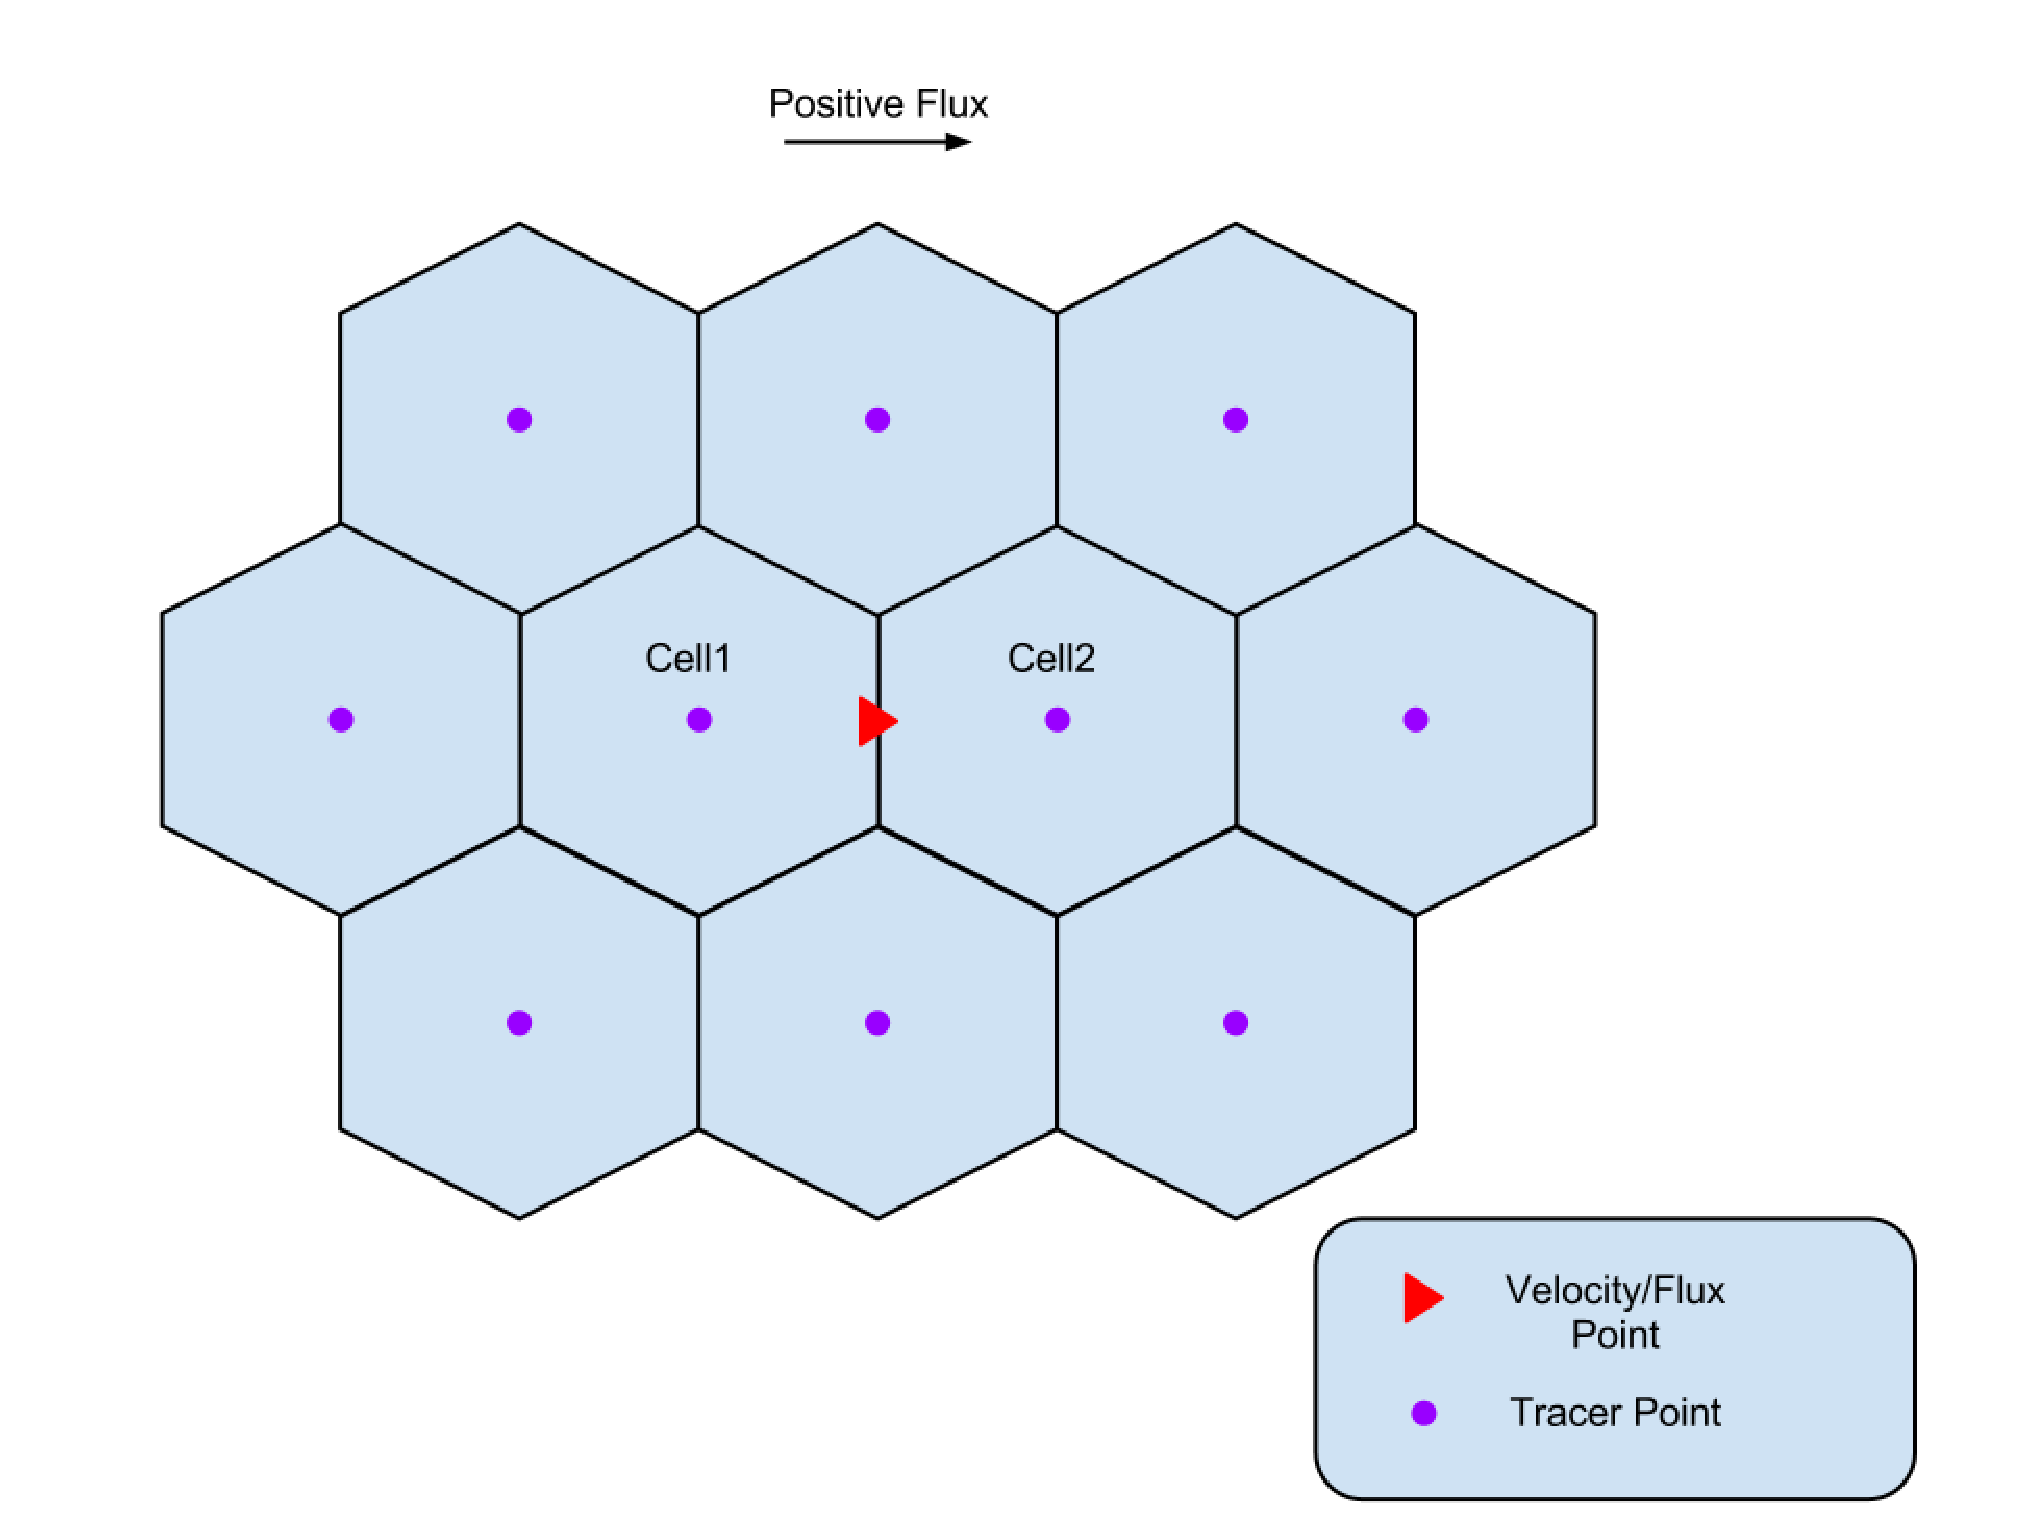
\includegraphics[scale=0.5]{HorizontalFluxDiagram.eps}
	\caption{Horizontal layout of cells. The triangle represents the edge where a flux will be computed, while the circles represent the location of the tracer values used to compute the flux.}
\end{figure}

Equation (\ref{eg:horiz_adv_cont}) can be discretized into the following form:
\begin{equation}
	q_i^{n+1} = \frac{1}{h^{n+1}}(h^n q_i^{n} + \frac{1}{A_j}\sum_{n_{e_j}} F_{e_j}(V_H, h, q_{j2})
\end{equation}
where $i$ the cell location that is being updated, $j$ represents the location across edge $j$ from cell $i$, $n$ represents a time level, and $F(V_H, h, q)$ represents a flux computation per unit length involving $q$ at an edge.

In general, $F(q)$ can be written as:
\begin{equation}
	F(V_H, h, q) = u h \tilde{q}
	\label{eq:flux_operator}
\end{equation}
where $u$ represents the horizontal velocity, called $V_H$ earlier, $h$ represents a thickness field, and $\tilde{q}$ represents a mapping of $q$ to the edge in of interest.

The all quantities in equation (\ref{eq:flux_operator}) live on edges. $h$ is mapped to an edge through a simple averaging using the two cells that share the edge, $u$ already lives on an edge, and the mapping of $q$ to $\tilde{q}$ (which lives on an edge) determines the type of advection scheme used.

The order of the advection scheme refers to the order of the flux divergence 

\subsection{1st order upwind advection }
The simplest choice of horizontal advection is a 1st order upwind biased scheme. This can be written as

\begin{equation}
	\tilde{q}_{h 1st} = \max(\frac{u}{|u|}, 0) * q_{i1} - \min(\frac{u}{|u|}, 0) * q_{i2}
\end{equation}

The choice of positve flux in this case is made as part of the requirements for MPAS grids, in that positive points from cell1 to cell2 along an edge.

\subsection{2nd order advection}
A second order advection scheme can be written as

\begin{equation}
	\tilde{q}_{h 2nd} = \frac{q_{i1} + q_{i2}}{2.0}
\end{equation}

\subsection{3rd and 4th order advection}
3rd and 4th order advection schemes are computed following (Skamarock and Gassman 2011) as

\begin{align*}
	\tilde{q}_{h 3rd} = &(\frac{1}{2}(q_{i1} + q_{i2}) - \frac{ dc^2}{12}(\frac{\delta^2 q}{\delta n^2}_{i2} + \frac{\delta^2 q}{\delta n^2}_{i1})  \\
                          &+ sign(u) \frac{ dc^2 \beta}{12}(\frac{\delta^2 q}{\delta n^2}_{i2} - \frac{\delta^2 q}{\delta n^2}_{i1}))
\end{align*} 

where $n$ represnets the normal direction to the edge shared by cells $i1$ and $i2$, $dc$ represents the distance between cell centers.

In this case, the second derivative of the tracer is required to implement a higher order advection scheme. These second derivatives are pre-computed using a least-squares method on a generic polynomial-fit in a tangent plane around the cell in question. These derivatives are stored in the array known as deriv\_two.

Using this general form, 3rd order advection is described as $\beta > 0$ and 4th order advection is when $\beta = 0$. Following (Skamarock and Gassman 2011) the optimal value is $\beta = 0.25$.

\section{Vertical Advection}
This section deals with vertical tracer advection, which can be described by the following equation.
\begin{equation}
	\frac{\partial h q}{\partial t} = - \frac{\partial (w h q)}{\partial z}
	\label{eq:cont_vert_adv}
\end{equation}

The figure below is used to show where different quantities from equation (\ref{eq:cont_vert_adv}) live on the vertical grid in MPAS.
\begin{figure}[H]
	\center
	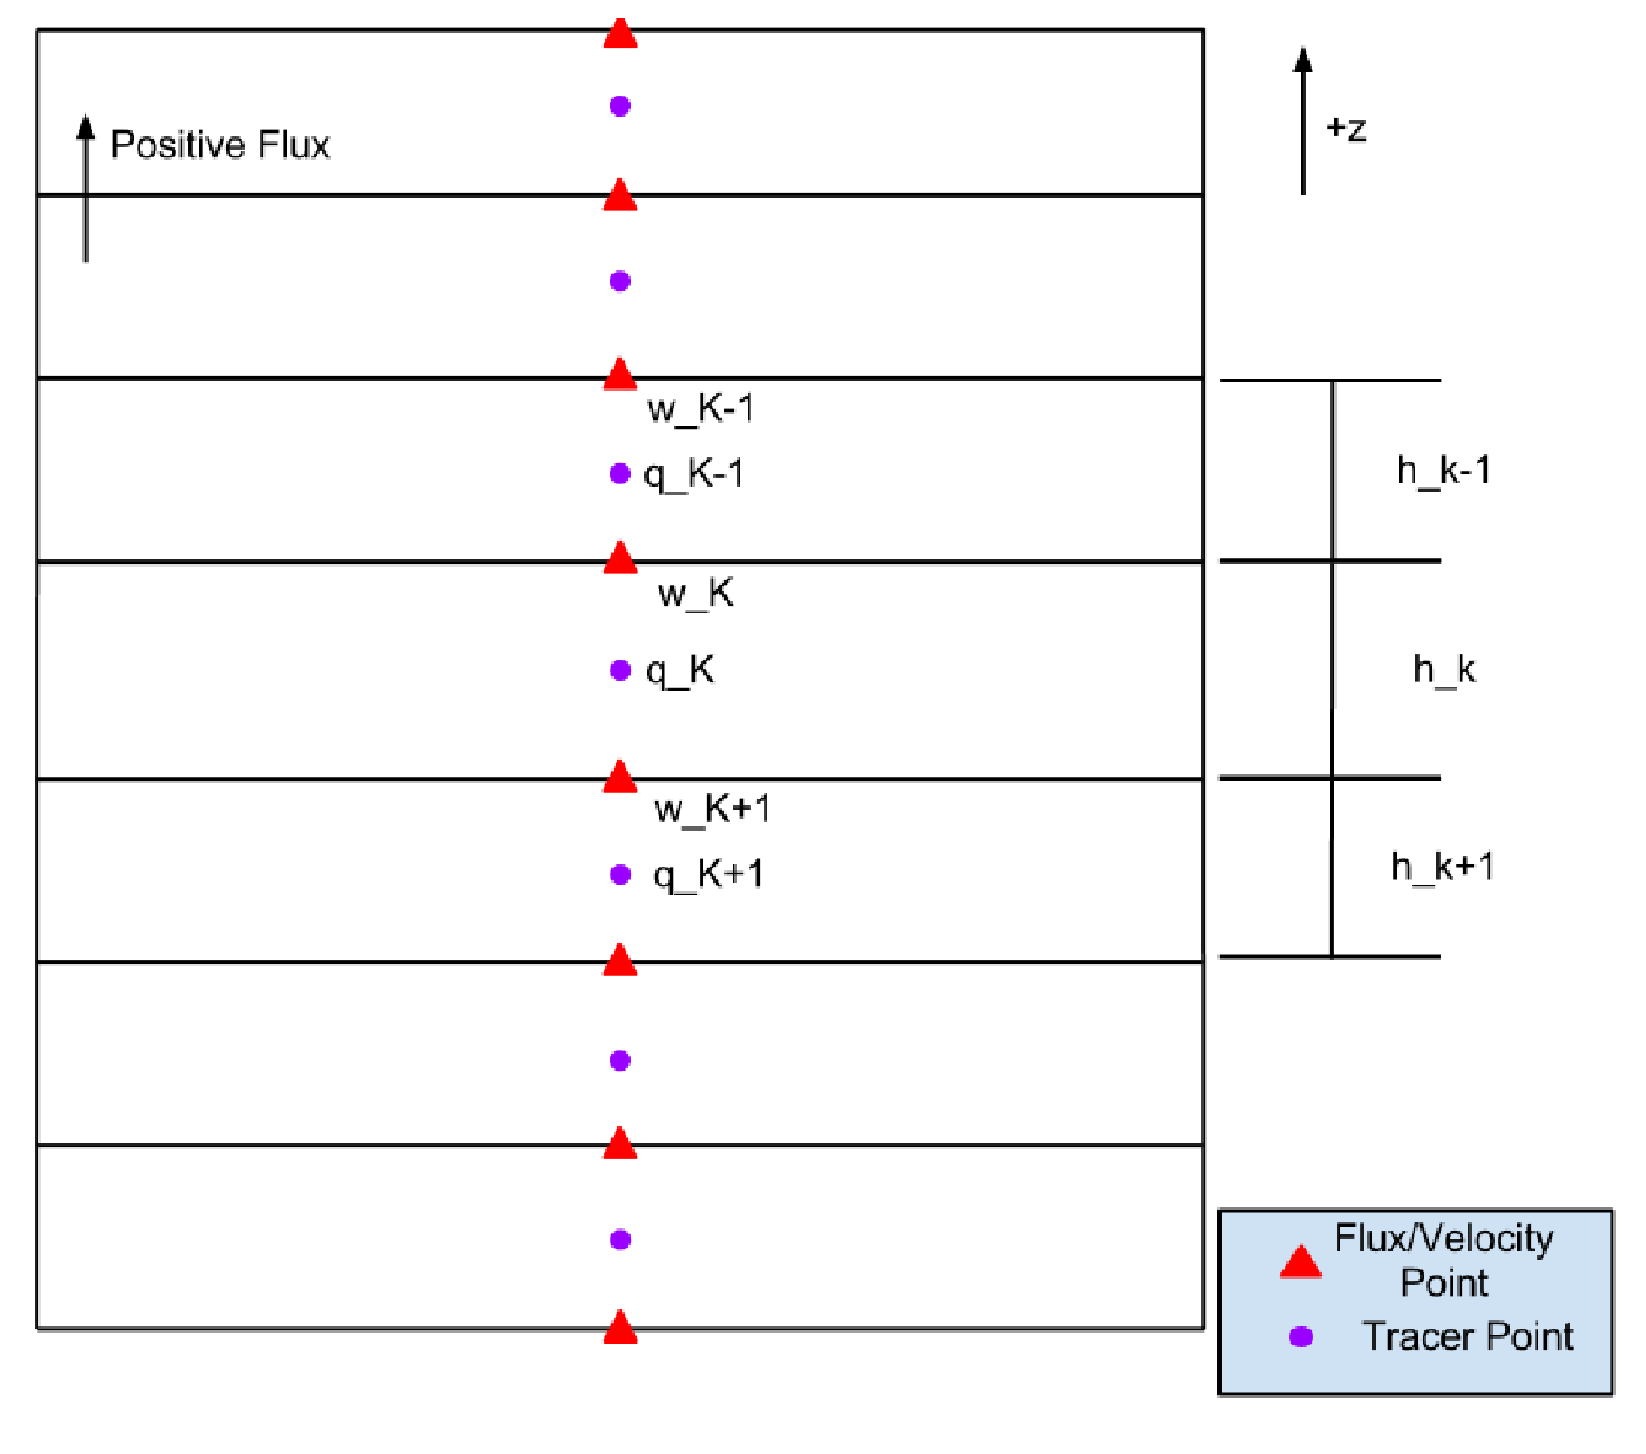
\includegraphics[scale=0.5]{VerticalFluxDiagram.eps}
	\caption{Diagram of vertical grid with velocity and flux points shown as red triangles, and tracer points shows as purple circles.}
	\label{fig:vert_flux_diagram}
\end{figure}

The discrete form of equation (\ref{eq:cont_vert_adv}) can be written as
\begin{equation}
	q_k^{n+1} = \frac{h^{n}q_k^{n} + \Delta t ( (F_z)_{k+1}^{n} - (F_z)_{k}^{n} )}{h^{n+1}}
\end{equation}
where $n$ represents a time level, $k$ represents a vertical level as seen in figure \ref{fig:vert_flux_diagram}, and $F_z$ represents the vertical flux across an interface.

In this equation, $q_k$ quantities live at vertical cell centers, and $(F_z)_k$ quantities live at vertical level interfaces.

$F_z$ can be written as:

\begin{equation}
	(F_z)_k = \tilde{q_k}(w_k)
\end{equation}

where $\tilde{q_k^n}$ represents an interpolated tracer value at interface $k$, and incorporates the factor of $h$ from (\ref{eq:cont_vert_adv}). The following subsections relate to different computations of $\tilde{q_k^n}$

\subsection{1st order upwind}
The 1st order upwind biased computation of $\tilde{q_k}$ is simply assigning $\tilde{q_k}$ with the upwind value of $q_k$, which can be written as:

\begin{align}
	c &= \frac{w_k}{|w_k|} \\
	\tilde{q_k}_{v 1st} &= \max(c,0)*q_{k} + \min(c,0)*q_{k-1}
\end{align}
\subsection{2nd order}
The 2nd order computation of $\tilde{q_k}$ involves a linear interpolation of q to an interface. This can be written as:
\begin{equation}
	\tilde{q_k}_{v 2nd} = \frac{h_k q_{k-1} h_{k-1} + q_{k}}{h_k + h_{k-1}}
\end{equation}
\subsection{3rd order}
The 3rd order computation of $\tilde{q_k}$ involves an interpolation of q to an interface based on the direction of the velocity at interface $k$. This can be written as:
\begin{align}
	c &= \frac{w}{|w|} \\
	\tilde{q_k}_{v 3rd} &= \frac{ (-1 + c) q_{k-2} + (7 - 3c) q_{k-1} + (7 + 3c) q_k + (-1 - c)q_{k+1}}{12.0}
\end{align}
\subsection{4th order}
The 4th order computation of $\tilde{q_k}$ involves an interpolation of q to an interface. This can be written as:
\begin{equation}
	\tilde{q_k}_{v 4th} = \frac{ 7(q_{k-1} + q_{k}) - 1(q_{k-2} + q_{k+1})}{12.0}
\end{equation}


\section{FCT - Monotonic Advection}
The FCT portion of tracer advection provides a blending of two types of fluxes in each direction, these consist of a low order flux (typically 1st order), and a higher order flux (typically 2nd, 3rd, or 4th order). The low order flux is chosen because it is monotonic. For the purposes of this section, we will introduce four fluxes, $F_{hl}$, $F_{hh}$, $F_{vl}$, and $F_{vh}$ which represent the horizontal low order, horizontal high order, vertical low order, and vertical high order respectively.

Each of the fluxes in this section can be computed using the methods in the previous sections, but for our purposes we will assume the following:
\begin{align*}
	F_{hl} &= u h \tilde{q_{h 1st}} \\
	F_{vl} &= u \tilde{q_{v 1st}}
\end{align*}

while the higher order fluxes can be computed using any of the remaining options. \\

To begin, bounds are computed in a cell by cell fashion. Each cell needs to contain the maximum and minimum value of $q$ taken from the set of itself and all cells it shares an edge with (either vertical or horizontal). We will call these $q_{max}^n$ and $q_{min}^n$ denoting these are at the current time step. \\

After these bounds are computed, the high order fluxes $F_{hh}$ and $F_{vh}$ are computed for each cell, or edge. \\

Next, the low order fluxes $F_{hl}$ and $F_{vl}$ are computed for each cell and edge, and their contribution is removed from $F_{hh}$ and $F_{vh}$. The remaining high order fluxes are stored on a cell by cell basis providing the high order perturbation fluxes. These new fluxes are stored in two arrays $\tilde{F_{in}}$ and $\tilde{F_{out}}$, the first being all fluxes incoming to a cell, and the second being all fluxes leaving a cell. \\

After the perturbation fluxes are constructed, scale factors are constructed. The scale factor $s$ represents the portion of the high order perturbation flux that can safely be used while still preserving monotonicity. It is computed by bounding the new flux value with the min and max values computed at the beginning of this section.

\begin{align}
	\hat{q^{n+1}}_{min} &= \frac{q^n*h^n + \Delta t * \tilde{F_{out}}}{h^{n+1}} \\
	\hat{q^{n+1}}_{max} &= \frac{q^n*h^n + \Delta t * \tilde{F_{in}}}{h^{n+1}} \\
	\hat{q^{n+1}}_{1st} &= \frac{q^n*h^n + \Delta t * (F_{hl} + F_{vl}}{h^{n+1}} \\
	s_{in} &= \frac{\hat{q^{n+1}}_{max}-\hat{q^{n+1}}_{1st}}{\hat{q^{n+1}}_{max}-\hat{q^{n+1}}_{1st}} \\
	s_{out} &= \frac{\hat{q^{n+1}}_{1st}-\hat{q^{n+1}}_{min}}{\hat{q^{n+1}}_{1st}-\hat{q^{n+1}}_{min}}
\end{align}

where the $\hat{q}$ values are incomplete predictions of $q$ at time level $n+1$. These are incomplete because they only include tendency updates caused from advection, and nothing else. $\Delta t$ in this step is the full time step.

Finally, the scale factors are applied to the perturbation fluxes in an upwind fashion to create the full flux across an edge.

\begin{align*}
	(F_{h})_{i} &= (F_{hl})_{i} \\
	&+ \max(0.0, (F_{hh})_{i} - (F_{hl})_{i}) * \min((s_{out})_{i1}, (s_{in})_{i2}) \\
	&+ \min(0.0, (F_{hh})_{i} - (F_{hl})_{i}) * \min((s_{in})_{i1}, (s_{out})_{i2}) \\
	(F_{v})_{k} &= (F_{vl})_{k} \\
	&+ \max(0.0, (F_{vh})_{k} - (F_{vl})_{k}) * \min((s_{out})_{k}, (s_{in})_{k-1}) \\
	&+ \min(0.0, (F_{vh})_{k} - (F_{vl})_{k}) * \min((s_{in})_{k} , (s_{out})_{k-1})
\end{align*}

where $i$ is an edge index, $i1$ and $i2$ are the indices of the cells that share edge $i$, and $k$ is a vertical index as shown in figure \ref{fig:vert_flux_diagram}.

\chapter{Pseudocode Formulation}
The monotonic advection routine can be written in pseudocode in the following form.
\begin{center}
	\line(1,0){250}
\end{center}
\begin{lstlisting}
Advect one tracer at a time:
  Determine bounds on tracer value at a cell. This involves the 
    minima and maxima of the current cell, and all cells that 
    share an edge with it (both horizontally and vertically)
    We call these q_min and q_max
	
  Compute 3rd order dispersive fluxes in vertical, and horizontal

  Compute 1st order diffusive upwind fluxes in vertical and 
    horizontal

  Removing the 1st order upwind component from the 3rd order flux, 
    compute a dispersive component of the flux. We will later scale 
	this portion of the high order flux in order to preserve 
	monotonicity.

  Determine scale factors.
    First, compute the maximum updated tracer value. This value 
      combines the previous value with all possible incoming fluxes 
      that postively contribute to it's value. We call this q_max_new

    Second, compute the minimum updated tracer value. This value 
      combines the previous value with all possible outgoing fluxes 
      that negatively contribute to it's value. We call this q_min_new

    Third, compute the upwind update tracer value. This value 
      combines the previous value with the 1st order upwind 
      tracer update value. We call this q_upwind_new

    Compute the two scale factors.
      scale_factor_in = 
        (q_max - q_upwind_new) / (q_max_new - q_upwind_new)
      scale_factor_out = 
        (q_upwind_new - q_min) / (q_upwind_new - q_min_new)

  Apply the newly computed scale factors to the remaining dispersive 
    flux components.

  Accumulate the upwind flux, and the scaled dispersive fluxes. These 
    provide a higher order monotonic flux.
\end{lstlisting}
\begin{center}
	\line(1,0){250}
\end{center}

\chapter{Design and Implementation}
In trying to implement the monotonic tracer advection these modules are placed
in src/operators. There are standard non-monotic advection routines and a
monotonic advection that are provided. This allows all cores to have shared
modules and a shared interface for advecting tracers.  \\

The previously described psuedocode is implemented in a monotonic advection module.\\

The advection routines are created within a driver framework, where the driver provides the following interfaces
\begin{lstlisting}[language=fortran,escapechar=@,frame=single]
subroutine mpas_ocn_tracer_advection_coefficients( grid, err )

subroutine mpas_ocn_tracer_advection_tend(tracers, uh, 
  w, h, verticalCellSize, dt, grid, tend_h, tend)

subroutine mpas_ocn_tracer_advection_init(err)
\end{lstlisting}

within this interface $uh$ defines a thickness weighted
velocity, $w$ is a vertical velocity, $h$ is a thickness field defined at cell
centers, $verticalCellSize$ defines the thickness of each vertical cell, 
$dt$ is the timestep over which advection is being performed,
$grid$ is the actual grid data structure, $tend_h$ is all tendencies on
the thickness field in order to update it to a new state, and $tend$ is the
tracer tendency array. \\

Within the driver module, various advection modules can be called. In the
default case, two submodules are provided one for monotonic advection using an
FCT and another for standard non-monotonic advection.

The mpas\_ocn\_tracer\_advection\_coefficients routine creates the coefficients
required to compute the high and low order horizontal fluxes. The
mpas\_ocn\_tracer\_advection\_init routine initializes some constants and
logicals for each of the advection modules. The
mpas\_ocn\_tracer\_advection\_tend routine is a driver routine that computes
the tendency cause from tracer advection.

\section{Namelist Options}

Within the new advection module there are several namelist options available.
This section will serve to describe each of them.

\begin{itemize}
	\item config\_vert\_tracer\_adv\_order \\
		This option determines the order of the flux reconstruction used for
		vertical advection. It is only used when the FCT is turned off. Within
		FCT advection only third or lower reconstuctions are used, and the user
		currently cannot choose the order. \\
		Available options include: 2, 3, 4
	\item config\_horiz\_tracer\_adv\_order  \\
		This option determines the order of the flux reconstuction used for
		horizontal advection. Contrary to the vertical advection, this is used
		in all cases. When the FCT is turned off this determines the only order
		that is used for advection. When the FCT is turned on, this determines
		the order that will be blended with the 1st order upwind flux. \\
		Available options include: 2, 3, 4
	\item config\_thickness\_adv\_order \\
		This option determines the order for the reconstruction of the
		thickness field to edges. \\
		Available options include: 2, 3, 4
	\item config\_coef\_3rd\_order \\
		This option sets the coefficient for $\beta$ in the horizontal
		advection equations above. It is only used when
		config\_horiz\_tracer\_adv\_order is equal to 3, and is overridded to
		be 0 when the horizontal order is chosen to be 4. \\
		Available options include: Any positive real number. Preferrably between 0 and 1. \\
		Optimal option: 0.25
	\item config\_monotonic \\
		This option enables or disables the FCT. \\
		Available options include: .true., .false.
	\item config\_check\_monotonicity
		This option provides a debugging mode where the model will check for
		monotonicity on each tracer field, on each time step. If the tracer is
		not monotonic the module returns an error flag which can be handled
		however the programmer wants. \\
		Available options include: .true., .false.
\end{itemize}

\chapter{Implementation Issues}

\section{Vertical Level Idexing}
In the atmosphere, every cell has nVertLevels levels. Because of this,
computations can span the entire column. However, in the ocean bottom
topography creates land cells which might be in the range of 1:nVertLevels.
Because of this, arrays are created as part of the grid structure called
maxLevelCell, maxLevelEdgeTop, and maxLevelEdgeBot. These represent the maximum
index of water cells in each column, the max index of an edge that has water
cells on both sides of it, and the max index of an edge that has at least one
water cell on eiter side of it.\\

In order to create a shared framework for tracer advection, all cores need to
have a shared method of changing the number of layers in a cell or on an edge. \\

The proposal to fix this issue is to implement a namelist flag called
config\_dzdk\_positive. This would have a default value of true in the
atmosphere, and false in the ocean. Other cores would need to specify their
value based on their grid structure. \\

This flag can be used to fix the following issue as well.

\section{Vertical Advection}
\subsection{Vertical Flux Directions}
There are issues present in all vertical advection sections. This is due to
indexing of vertical levels. In the atmosphere, k is indexed positively as
cells move upwards. Because of this, positive vertical fluxes occur in
direction of increasing k. In the ocean, k is index positively as cells move
downwards, so vertical fluxes are positive in the direction of decreasing k.
This needs to be accounted for if the routines are to be shared across cores.
\subsection{flux3 mapping}
\subsubsection{MPAS-O}
To begin, the tracerTop array is filled. When applicable a 3rd order stencil is used. The stencil for 3rd order is written as follows.

\begin{align*}
	tracerTop = &((-1 + C) * q_{k-2} \\
	            &+(7- 3*C) * q_{k-1} \\
				&+(7+ 3*C) * q_{k} \\
				&+(-1 - C) * q_{k+1})/12.0
\end{align*}

Expanding this, we arrive at the following form.

\begin{align*}
	tracerTop &= ((-q_{k-2} + C*q_{k-2}) \\
		       &+ (7*q_{k-1} - 3*C*q_{k-1}) \\
			   &+ (7*q_{k} + 3 * C * q_{k}) \\
			   &+ (-1 * q_{k+1} - C*q{k+1}))/12.0
\end{align*}

\subsubsection{Atmosphere}
In the atmosphere a 3rd order stencil is used to compute vertical fluxes. This stencil is written as follows.

\begin{align*}
	flux3 &= (u * (7 * (q_{k} + q_{k-1}) - (q_{k+1} + q_{k-2})) \\
		  &+C * |u| *((q_{k+1}-q_{k-2}) - 3 * (q_{k} - q_{k-1})))/12.0
\end{align*}

If we try to refactor this to arrive at a similar expression as in the MPAS-O section we find the following form:

\begin{align*}
	flux3 &= ((-u * q_{k-2} - C * |u| * q_{k-2}) \\
		  &+  ( u * 7 * q_{k-1} + 3 * C * |u| * q_{k-1}) \\
		  &+  ( u * 7 * q_{k}   - 3 * C * |u| * q_{k}) \\
		  &+  (-u * q_{k+1} + C * |u| * q_{k+1})) / 12.0
\end{align*}

\section{Nomenclature}
There are differences in each community for the name of tracers, or scalars. It seems that the atmospheric cores call them scalars, whereas the ocean core calls them tracers. In order for these routines/modules to be shared between all cores a name needs to be agreed upon between all cores. \\

This is due to the tracer super array being passed in, so the tracer super array requires the same name between all cores. \\

An alternative method to solving this issue, is to pass in a single tracer to advect, and having a loop over tracers outside the call to this module.
\end{document}

